\section*{Interazione geni-ambiente}
<<<<<<< HEAD
 \subsection{Introduzione}
 Questo esperimento valuterà la qualità della trasmissione del DNA, ma concentrandosi sui meccanismi di riparazione dello stesso in diverse condizioni ambientali, piuttosto che prendere ad esempio la sola replicazione, come nelle esperienze precedenti. Si cercherà di comprendere le eventuali esposizioni ambientali su di un gene e la bontà della replicazione del DNA, focalizzandosi su errori di replicazione che vengono - o non vengono - riparati. 
 
 \subsubsection{}
 Può succedere in vivo che una polimerasi catalizzi il nucleotide sbagliato durante il processo di replicazione, ma questa non viene considerata come una mutazione perché questo errore può essere ancora riconosciuto e risolto. I due modi in cui una cellula ripara i \textit{mismatch} sono l'attività di proofreading polimerasica, ed il sistema di riparazione dei mal appaiamenti (MMR). Volendo studiare mutazioni causate da mismatch, a questo punto sorge un'ambiguità: la mutazione potrebbe essere stata causata dal fallimento dell'attività esonucleasica della polimerasi, da un errore nel nucleotide incorporato erroneamente o del DNA \textit{mismatch repair} (MMR). 
 
 \subsubsection{}
 Si è costruito un sistema che permettesse di superare l'ambiguità causata da questa doppia linea di difesa contro i mal appaiamenti. Si è visto che in sequenze omonucleotidiche la polimerasi tende ad introdurre un nucleotide in più, anche a causa di una potenziale diversa topologia assunta dai due filamenti di DNA in presenza di lunghe sequenze ripetute. Se la sequenza omonucleotidica da copiare è ricca soprattutto in A e T e diventa lunga, precisamente maggiore di 7, la correzione di bozze sembra essere totalmente inefficace. Rimane quindi un solo meccanismo di riparazione, MMR appunto, ed è su questa osservazione che si basa il nostro esperimento. 
 
 Non tutte le sequenze di DNA sono replicabili con la stessa efficacia, quelle che potrebbero rappresentare siti di mutazione vengono chiamate \textit{at risk motifs}.  Vogliamo testare, sfruttando queste sequenze più fragili, se alcune condizioni nel terreno, come agenti mutageni, possono interferire con il sistema MMR. Per farlo in vivo abbiamo bisogno di un saggio reporter, nel nostro caso un gene importante nella biosintesi della lisina, il gene \textit{LYS2}. Avremo a disposizione un ceppo il quale è stato precedentemente sottoposto ad un intervento di ingegnerizzazione, nel quale il gene \textit{LYS2} è stato inattivato da uno \textit{stretch} omonucleotidico di 14 A. Il quadro di lettura del nostro ceppo sarà quindi sfalsato a valle a causa delle 13 adenine esogene, inserite per altro al centro del gene, impedendo al ceppo di vivere in un terreno senza lisina. Oltre al ceppo che in questo esperimento chiamiamo \textit{wild type} (WT), si sono sfruttati altri tre ceppi: $\delta$msh2, nel quale è stato inattivato il gene \textit{msh2}, $\delta$msh6 nel quale è stato reso inattivo il gene \textit{mlh1} ed infine, $\delta$msh6, con gene \textit{msh6} spento. Di seguito si riportano i genotipi. \\
WT\textit{(MATalpha, ade5-1 his 7-2 leu 2-3, 112 trp1-289 ura3-52 lys2::insE-A14)} \\
$\delta$msh2(isogenico al WT tranne per la \textit{msh2::kanMX}) \\
$\delta$mlh1(isogenico al WT tranne per la \textit{mlh1::kanMX}) \\
$\delta$msh6(isogenico al WT tranne per la \textit{msh6::kanMX})
 
 
 \subsection{•}
 La preparazione all'esperimento si è svolto nell'arco dei tre giorni. Per prima cosa, partendo dalle colonie di ciascun ceppo di lievito fornite, si sono preparate due \textit{patches} su una piastra YPDA, seguendo lo schema riportato sul protocollo, usando stecchi sterili. Si è lasciato incubare a 30 C° durante la notte. Il giorno dopo le piastre con i \textit{patches} di ceppi mutanti sono state replicate su cinque diverse piastre. Una piastra con un terreno SD complete, da usare come controllo; un'altra con SD lys, deficiente di lisina; altre due piastre SD lys CdCl$_{2}$, rispettivamente con una dose di cadmio cloruro di 0.5$\mu$M e 5$\mu$M; un'ultima piastra contente SD his, un terreno privo di istidina. Si sono lasciate queste piastre ad incubare a 30 C° e quattro giorni dopo si è potuto apprezzare il risultato.
 
 \subsection{Risultati ottenuti}
	Come ci aspettavamo, nella piastra contenente un media completo (piastra 4.) tutti i diversi ceppi sono cresciuti senza rilevazione di sostanziali differenze. Nella piastra con terreno senza lisina (piastra 5.) possiamo invece osservare che il ceppo WT non è riuscito a crescere, con apparizione di 17 colonie. I ceppi $\delta$msh2 e $\delta$mlh1 hanno visto una crescita importante, mentre il ceppo $\delta$msh6 leggermente minore alle due precedenti. Un risultato molto simile, con una differenza di quantità di colonie sostanziale solo per WT, è stata registrata per la piastra con una dose di cadmio cloruro pari a 0,5$\mu$M (piastra 1) e per quella contente 5$\mu$M di CdCl$_{2}$. Una differenza visibile tra le due piastre contenenti CdCl$_{2}$ e quella SD lys è che le colonie nelle prime due sono leggermente più piccole, anche se in numero maggiore. Diversamente dalle altre, la piastra in cui era assente l'istidina, ha visto una crescita minima di tutti di ceppi: crescita nulla per WT, appena una 20ina di colonie per \textit{patch} per i ceppi $\delta$msh2 e $\delta$mlh1. 
	
 \begin{figure}[H]
	\centering
    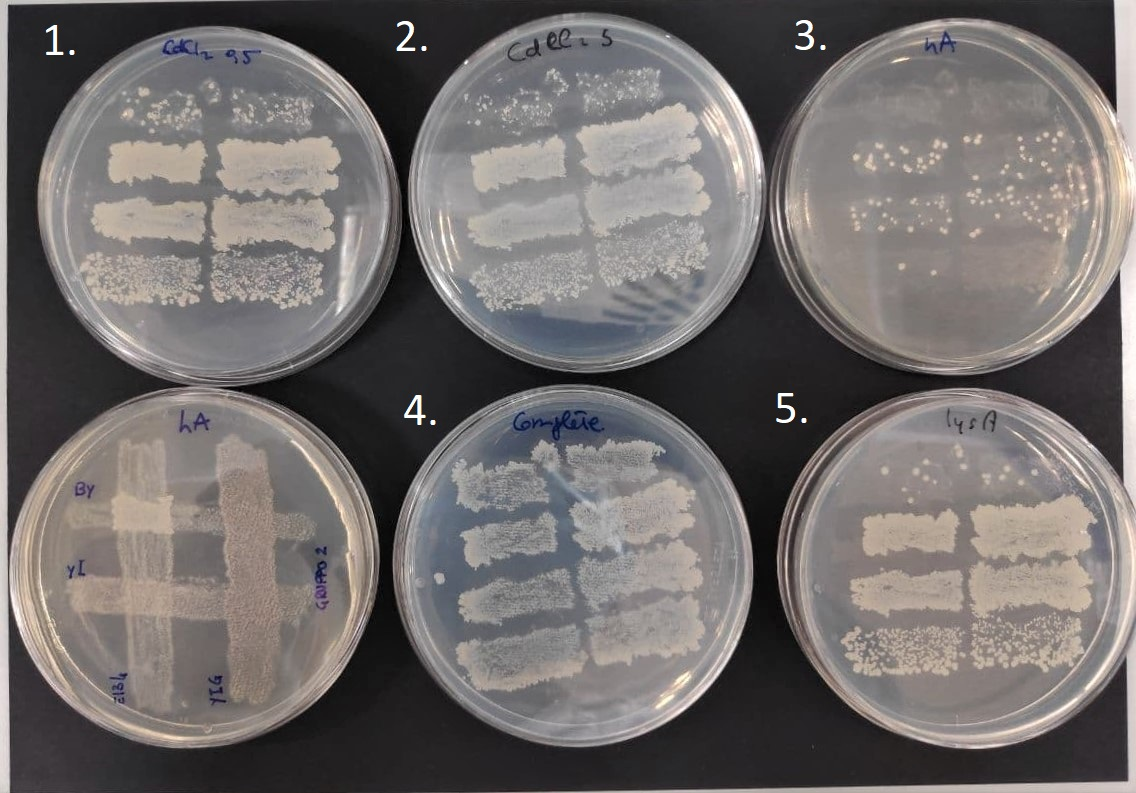
\includegraphics[scale=0.4]{./Pics/geneambientemod1.jpg}
	\caption{Colonie di ceppi mutanti cresciuti su piastre con terreni diversi}
	\label{fig1}
	\end{figure}
 
 
 \subsection{Conclusioni}
 
 Il ceppo nella prima linea di ogni piastra è il ceppo WT, di cui si è discusso ampiamente all'inizio di questa sezione. Il motivo per cui WT non riesce a crescere in un terreno privo di lisina è lo shift del quadro di lettura causato dall'inserimento di 13 adenine. Se però ci fosse un errore di sintesi del DNA, nella quale la polimerasi lascia indietro una adenina, si avrebbe una discendenza nella quale le cellule hanno 12 adenine esogene, restaurando il quadro di lettura mantenendo le stesse triplette in tutto il genoma a valle dell'inserzione e il mutante tornerebbe a crescere in un terreno senza lisina. Questo effetto lo si vede in ogni piastra nella prima riga con l'apparizione di colonie revertanti. Affinché la cellula si "lasci sfuggire" un nucleotide, ha però bisogno La quantificazione della reversione del gene \textit{LYS2} consente di stimare il numero di mal appaiamenti risolti grazie a MMR.
 
 
=======
\subsection*{Introduzione}
Questo esperimento valuterà la qualità della trasmissione del DNA, ma concentrandosi sui meccanismi di riparazione dello stesso in diverse condizioni ambientali, piuttosto che prendere ad esempio la sola replicazione, come nelle esperienze precedenti. 
Cercheremo di comprendere le eventuali esposizioni ambientali su di un gene e la bontà della replicazione del DNA, focalizzandoci su errori di replicazioni che vengono o non vengono riparati. 

 \subsubsection*{}
 Può succedere in vivo che una polimerasi catalizzi il nucleotide sbagliato durante il processo di replicazione, ma questa non viene considerata come una mutazione perché questo errore può essere ancora riconosciuto e risolto. 
I due modi in cui una cellula ripara i cosiddetti "mal appaiamenti" o "mismatch", sono, da una parte, l'attività esonucleasica intrinseca alla polimerasi, dall'altra il sistema di riparazione dei mal appaiamenti. 
Se si vogliono studiare mutazioni causate da mismatch, a questo punto sorge un'ambiguità. 
La mutazione potrebbe essere stata causata dal fallimento dell'attività esonucleasica della polimerasi, da un errore nel nucleotide incorporato erroneamente o del DNA \textit{mismatch repair} (MMR). 

 \subsubsection*{}
 Si è costruito un sistema che permettesse di superare l'ambiguità causata da questa doppia linea di difesa contro i mal appaiamenti. 
Sì è visto che in sequeunze omonucleotidiche la polimerasi tende ad introdurre un nucleotide in più, anche a causa di una potenziale diversa topologia assunta dai due filamenti di DNA in presenza di lunghe sequenze ripetute. 
Se la sequenza da copiare omonucleotidica, soprattutto A e T diventa lunga, maggiore di 7, la correzione di bozze sembra essere totalmente inefficace, la polimerasi non si rende conto di absi extraelica che dà una distorsione dell'elica, già uscita dal sito catalitico. 
Rimane un solo meccanismo di riparazione, MMR appunto, ed è su questa osservazione che si basa il nostro esperimento. 

 
 \subsection*{Risultati}
 Non tutte le sequenze di DNA sono replicabili con la stessa efficacia, quelle che potrebbero rappresentare siti di mutazione vengono chiamate \textit{at risk motifs}. 
 Vogliamo testare, sfruttando queste sequenze più fragili se alcune condizioni nel terreno, come agenti mutageni, possono interferire con il sistema MMR. 
Per farlo in vivo abbiamo bisogno di un saggio reporter, nel nostro caso un gene importante nella biosintesi della lisina. 
Avremo a disposizione un ceppo il quale è stato sottoposto ad un intervento di ingegnerizzazione, non fatto da noi am ereditato, nel quale il gene \emph{lys2} è stato inattivato da uno stretch omonucleotidico di $A$ (precisamente $14$). 
Le $A$ effettivamente inserite sono comunque $13$. 
Scivolamento del modulo di lettura bisogna interpretarlo come uno shift di $13$ A. 
Il quadro di lettura del nostro ceppo sarà quindi sfalsato a valle. 
dato che è posizionato abbastanza al centro della sequenza codificante, il nostro ceppo non sarà più in grado di crescere in un terreno senza lisina. 
Noi partiremo da un reporter che ha bisogno di lisina per crescere su piastra. 
Ma se ci fosse un errore di sintesi del DNA, nella quale la polimerasi lascia indietro una adenina, ecco che avremmo una discendenza nella quale le cellule hanno 12 adenine esogene, restaurando il quadro di lettura. 
Il mutante tornerà a crescere in un terreno senza lisina. 
Vederemo apparire effetto della reversione. 
La quantificazione della reversione ci consente di stimare il numero di malappaiamenti risolti grazie a MMR.
 
 \subsection*{Considerazioni finali}
 La preparazione all'esperimento si è svolto nell'arco dei tre giorni. 

>>>>>>> 377d60ee9b1d76b51ddc46b5ab46846c0d43637f
